Dans ce manuscrit, vous trouverez l'ensemble des résultats de mes travaux de thèse, mais avant de présenter ceux-ci, je vais ici introduire le contexte dans lequel j'ai effectué ces travaux.
Je suis issu d'une formation en informatique fondamentale de Lille 1 et spécialisé en algorithmique par un master de cette même université.
C'est dans le cadre de mon parcours universitaire que j'ai eu l'occasion de rencontrer Maude Pupin et Laurent Noé, mes actuels directeurs de thèse.
Ils m'ont accueilli plusieurs fois en projets de master et stages, puis en thèse au sein de l'équipe Bonsai dirigée par Hélène Touzet, équipe de bioinformatique à cheval sur le laboratoire CRIStAL et INRIA.

L'équipe Bonsai est une équipe de bioinformatique orientée algorithmique.
Plus précisément, l'équipe est orientée algorithmique des séquences, qu'elles soient ARN, ADN, de gènes ou moléculaires.
Ma thématique de recherche est elle orientée structures moléculaire pour des molécules appelées peptides non ribosomiques.
Au cours de mes 3 années de thèse j'ai interagi à de nombreuses reprises avec d'autres thématiques de l'équipe, mais deux discutions ont particulièrement menées à des collaborations hors de mon cadre de recherche usuel.

\begin{figure}[!ht]
  \begin{center}
    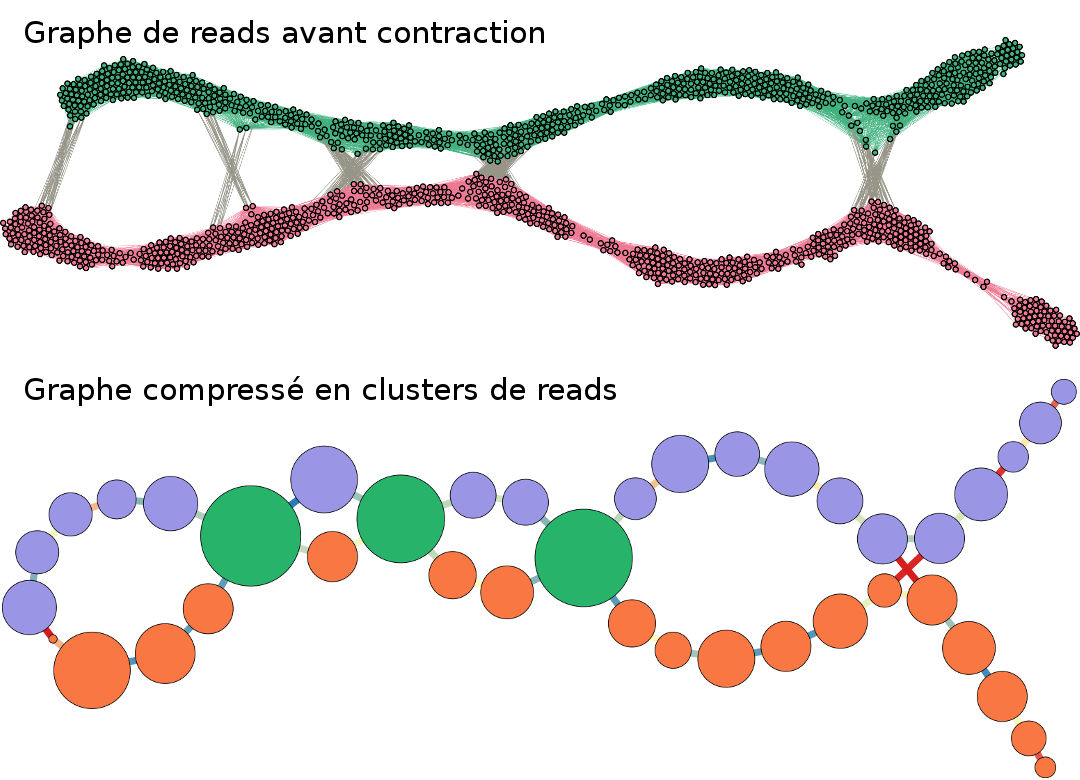
\includegraphics[width=350px]{Figures/preambule/pierre.png}
    \caption{\label{pierre}Contraction d'un graphe de read pour extraire les clusters à assembler ensuite.
    Ces données sont issues d'un métagénome simple à deux espèces.}
  \end{center}
\end{figure}

Pierre Péricard est un doctorant de l'équipe qui travaille sur un pipeline d'assemblage de marqueurs conservés dans des données métagénomiques.
Durant le déroulement algorithmique du programme, il est amené à construire un graphe de reads présents dans l'échantillon où deux reads sont liés lorsqu'ils sont partiellement chevauchants (voir figure \ref{pierre}).
Il souhaitait pouvoir extraire les composantes ``linéaires'' pour effectuer des assemblages sur ces sous-jeux de read.
J'ai créé pour lui un programme qui permet de réduire ce graphe avec une épaisseur en un graphe filiforme facilement découpable au niveau des arêtes faibles (en rouge sur la figure) et des noeuds d'arité supérieure à 2.
Cet utilitaire permet la contraction des noeuds proches via des distances calculées par l'algorithme de Dijkstra, ainsi que l'utilisation de plusieurs filtres discriminant les reads ne contribuant pas à l'homogénéité du graphe.
Le pipeline complet sera prochainement publié par Pierre.

En début d'année, Hélène Touzet a publié un article contenant une méthode de programmation dynamique permettant le comptage des voisins d'un mot avec k erreurs.
Cette méthode utilise le croisement de deux automates dont l'un est l'automate universel déterministe de Levenshtein.
Le fait que cet automate ne dépende pas du mot dont on va regarder le voisinage, permet de le générer une seule fois et permet de n'avoir plus qu'à le croiser avec le second automate lors de chaque exécution.
Depuis cette publication, je me suis proposé pour travailler avec Hélène sur l'implémentation de la méthode puis sur l'analyse de la minimalité de l'automate universel déterministe de Levenshtein que nous avons généré.
Ces travaux sont en cours et feront l'objet du publication prochaine.

~~

Mon sujet de thèse m'a également amené à collaborer avec de nombreuses personnes locales mais également d'équipes distantes.
Localement, j'ai travaillé avec plusieurs membres de l'institut Charles Violette, institut également hébergé par l'université Lille 1.
J'ai notamment beaucoup travaillé avec Valérie Leclère pour les aspects biologie de mon sujet et Mickael Chevalier pour les aspects spectrométrie de masse.

À l'extérieur, j'ai principalement travaillé avec Tilmann Weber et son équipe hébergée au Danemark par la Novo Nordist Foundation.
Ses travaux sur l'outil Antismash en font un collaborateur de longue durée au sein de la thématique des peptides non ribosomiques sur l'université Lille 1.
C'est d'ailleurs cette collaboration entre son équipe et la notre qui a permis l'organisation, à Lille et par deux fois (en 2013 et 2015), d'un workshop sur la thématique des outils bioinformatiques pour l'analyse des peptides non ribosomiques et des polykétides.
Cette collaboration de longue date m'a également permis d'être accueilli durant un mois au Danemark dans son équipe pour démarrer avec son équipe, le développement d'une nouvelle application dont nous parlerons dans la partie \ref{bio_synth} de ce manuscrit.

Depuis maintenant plus d'un an, l'équipe autour de Norine est également en collaboration avec l'équipe de recherche Suisse ``Proteome Informatics'' dirigée par Frédérique Lisacek, dans le but de créer un pipeline d'identification de NRP via spectrométrie de masse.
Deux doctorants ont été recruté à Lille (Mickael Chevalier) et Genève (Emma Ricart).
Durant ma thèse, j'ai collaboré avec Emma pour son utilisation de smiles2monomers (logiciel développé durant ma thèse) afin de valider les structures biologiques de ses peptides non ribosomiques.

~~

Globalement, mon contexte de travail a été particulièrement agréable et m'a permis de m'ouvrir l'esprit à la recherche mais également à la vie universitaire en générale.
Les 3 ans et 6 mois d'enseignement en informatique et les différentes responsabilités universitaires, telles que la création et gestion d'un groupe d'entrainement algorithmique avec Thibault Raffaillac, m'ont préparé à l'éventualité de devenir un jour maître de conférence ou chercheur.



























